\documentclass[a4paper]{article}
\usepackage[utf8]{inputenc}
\usepackage[spanish, es-tabla]{babel}

\usepackage{amsmath}
\usepackage{amsfonts}
\usepackage{amssymb}

\usepackage{float}
\usepackage{graphicx}
\graphicspath{ {./Imagenes/} }

\usepackage[american voltage]{circuitikz}

\usepackage{fancyhdr}

\usepackage{units} 

\pagestyle{fancy}
\fancyhf{}
\lhead{22.02 Electrotecnia I}
\rhead{Mechoulam, Mestanza, Lambertucci, Pouthier, Londero}
\rfoot{Página \thepage}



\begin{document}

%%%%%%%%%%%%%%%%%%%%%%%%%%%%%%%%%%%%%%%%%%%%%%%%%%%%%%%%%%%%%%%%%%%%%%%%% 
%								CARATULA								%
%%%%%%%%%%%%%%%%%%%%%%%%%%%%%%%%%%%%%%%%%%%%%%%%%%%%%%%%%%%%%%%%%%%%%%%%% 

\begin{titlepage}
\newcommand{\HRule}{\rule{\linewidth}{0.5mm}}
\center
\mbox{\textsc{\LARGE \bfseries {Instituto Tecnológico de Buenos Aires}}}\\[1.5cm]
\textsc{\Large 22.02 Electrotecnia I}\\[0.5cm]


\HRule \\[0.6cm]
{ \Huge \bfseries Trabajo práctico N$^{\circ}$3}\\[0.4cm] 
\HRule \\[1.5cm]


{\large

\emph{Grupo 5}\\
\vspace{3px}

\begin{tabular}{lr} 	
\textsc{Mechoulam}, Alan  &  58438\\
\textsc{Lambertucci}, Guido Enrique  & 58009 \\
\textsc{Pouthier}, Florian  & 61337 \\
\textsc{Mestanza}, Nicolás  & 57521 \\
\textsc{Londero Bonaparte}, Tomás Guillermo  & 58150 \\
\end{tabular}

\vspace{20px}

\emph{Profesores}\\
\vspace{3px}
\textsc{Muñoz}, Claudio Marcelo\\ 	
\textsc{Ayub}, Gustavo\\ 	

\vspace{100px}

\begin{tabular}{ll}

Presentado: & 17/05/19\\

\end{tabular}

}

\vfill

\end{titlepage}


%%%%%%%%%%%%%%%%%%%%%%%%%%%%%%%%%%%%%%%%%%%%%%%%%%%%%%%%%%%%%%%%%%%%%%%%% 
%								INFORME									%
%%%%%%%%%%%%%%%%%%%%%%%%%%%%%%%%%%%%%%%%%%%%%%%%%%%%%%%%%%%%%%%%%%%%%%%%%

\section*{Introducción}

En la experiencia realizada se buscó analizar las potencias reactivas, activas y aparentes en los distintos tipos de circuitos propuestos. Para ello se valió del uso de un amperímetro, un voltímetro y un vatímetro, puestos en serie con la fuente, en paralelo y de ambas formas, respectivamente.

\section*{Desarrollo de la experiencia}

\subsection*{\underline{Ejercicio 1}}

En esta etapa, se analizó un circuito con una bobina, la cual dispone de un núcleo de hierro macizo, lo que permitió observar tres situaciones distintas:
\begin{enumerate}
	\item[A)] La totalidad del núcleo dentro de la bobina.
	\item[B)] La mitad del núcleo dentro de la bobina.
	\item[C)] Sin núcleo.
\end{enumerate}

\begin{figure}[H]
	\centering
	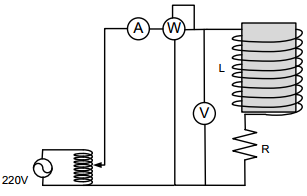
\includegraphics[width=0.6\textwidth]{Circuito-ejercicio-1A}
	\caption{Circuito con la totalidad del núcleo dentro de la bobina.}
	\label{fig:1a}
\end{figure}

\begin{figure}[H]
	\centering
	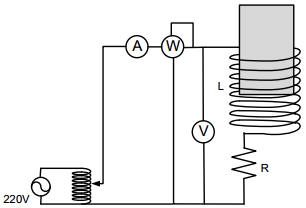
\includegraphics[width=0.6\textwidth]{Circuito-ejercicio-1B}
	\caption{Circuito con la mitad del núcleo dentro de la bobina.}
	\label{fig:1b}
\end{figure}

\begin{figure}[H]
	\centering
	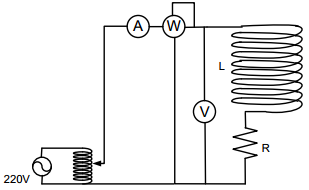
\includegraphics[width=0.6\textwidth]{Circuito-ejercicio-1C}
	\caption{Circuito con sin núcleo.}
	\label{fig:1c}
\end{figure}

De las mediciones realizadas, se pudo confeccionar la siguiente tabla:

\begin{table}[H]
\centering
\begin{tabular}{|c|c|c|c|c|c|c|}
\hline
\textbf{Circuito}                                                       & \textbf{P {[}W{]}} & \textbf{I {[}A{]}} & \textbf{V {[}V{]}} & \textbf{Q {[}VAR{]}} & \textbf{S {[}VA{]}} & \textbf{Cos($\varphi$)} \\ \hline
A) Núcleo sólido                                                        & 7,25               & 0,28               & 99,50              & 26,38                & 27,36               & 0,26                                \\ \hline
\begin{tabular}[c]{@{}c@{}}B) Núcleo sólido\\ por la mitad\end{tabular} & 9,88               & 0,46               & 98,50              & 43,72                & 44,82               & 0,22                                \\ \hline
C) Sin núcleo                                                           & 23,25              & 0,92               & 96,00              & 85,40                & 88,51               & 0,26                                \\ \hline
\end{tabular}
\caption{Tesiones, corrientes y potencias medidas y calculadas.}
\label{table:ej1}
\end{table}

A continuación se procede a graficar, para cada circuito, un diagrama fasorial de la corriente y la tensión:

\begin{figure}[H]
\centering
\begin{minipage}{.5\textwidth}
	\centering
	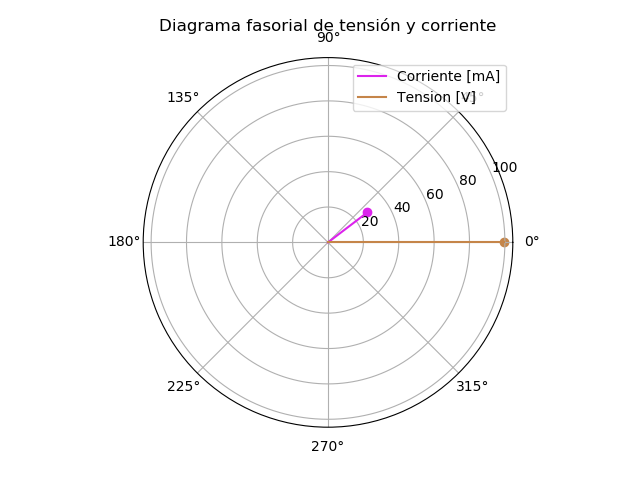
\includegraphics[width=1.2\linewidth]{Fasorial-1A.png}
	\caption{Fasores del circuito A.}
	\label{fig:faso-1a}
\end{minipage}
\begin{minipage}{.5\textwidth}
	\centering
	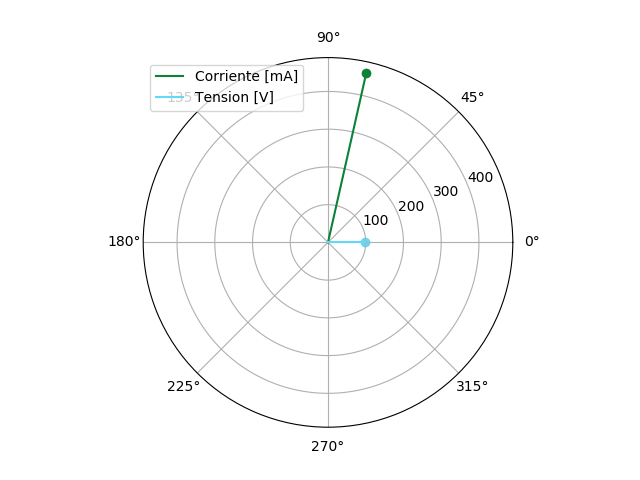
\includegraphics[width=1.2\linewidth]{Fasorial-1B.png}
	\caption{Fasores del circuito B.}
	\label{fig:faso-1b}
\end{minipage}\\
\end{figure}

\begin{figure}[H]
\centering
\begin{minipage}{.5\textwidth}
	\centering
	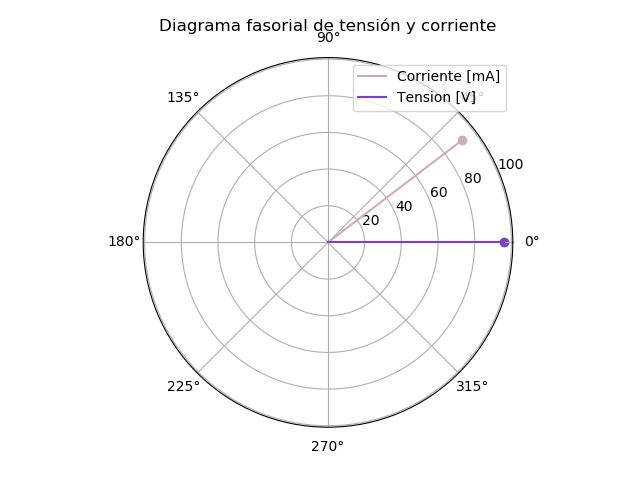
\includegraphics[width=1.2\linewidth]{Fasorial-1C.png}
	\caption{Fasores del circuito C.}
	\label{fig:faso-1c}
\end{minipage}
\end{figure}

Finalmente, analizando los resultados obtenidos se puede observar que al retirar el núcleo metálico, la inductancia baja, aumentando la potencia activa del circuito. Por otra parte, esto aumenta la corriente, lo que genera un crecimiento tanto de la potencia reactiva como aparente. Por último, cabe destacar que el factor de potencia se mantiene prácticamente inalterado en los casos A) y B). Se atribuye dicho error a la poca diferencia entre la resistencia y la reactancia.

\subsection*{\underline{Ejercicio 2}}

En la segunda etapa se medió la potencia activa, reactiva y aparente, junto al valor del $Cos(\varphi)$ de tres circuitos diferentes: R, C, y RLC.

\begin{figure}[H]
\centering
\begin{minipage}{.5\textwidth}
  \centering
  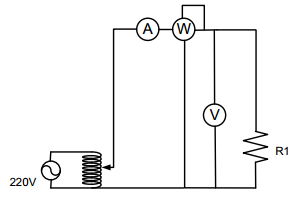
\includegraphics[width=.8\linewidth]{Circuito-ejercicio-2A}
  \caption{Circuito R}
\end{minipage}%\\
\begin{minipage}{.5\textwidth}
  \centering
  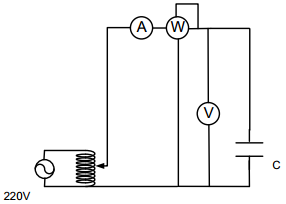
\includegraphics[width=.8\linewidth]{Circuito-ejercicio-2B}
  \caption{Circuito C}

\end{minipage}%\\
\end{figure}
\begin{figure}[H]
\centering
\begin{minipage}{.5\textwidth}
  \centering
  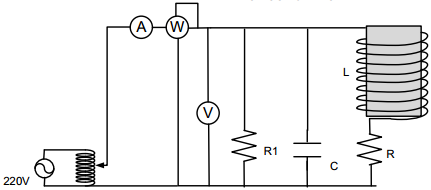
\includegraphics[width=.8\linewidth]{Circuito-ejercicio-2C}
  \caption{Circuito RLC}
  \label{fig:2b}
\end{minipage}
\end{figure}

Obteniendo, los siguientes valores:

\begin{table}[H]
\centering
\begin{tabular}{|c|c|c|c|c|}
\hline
\textbf{Circuito} & \textbf{P {[}W{]}} & \textbf{Q {[}VAR{]}} & \textbf{S {[}VA{]}} & \textbf{Cos($\varphi$)} \\ \hline
R                 & 54,5               & 6,23                 & 54,5                & 0,99                                \\ \hline
C                 & 9,38               & 106,09               & 9,38                & 0,09                                \\ \hline
RLC               & 0,74               & 78,01                & 86                  & 0,74                                \\ \hline
\end{tabular}
\caption{Valores medidos de potencia.}
\end{table}

Graficando fasorialmente las tres potencias, se obtienen:

\begin{figure}[H]
\centering
\begin{minipage}{.5\textwidth}
  \centering
  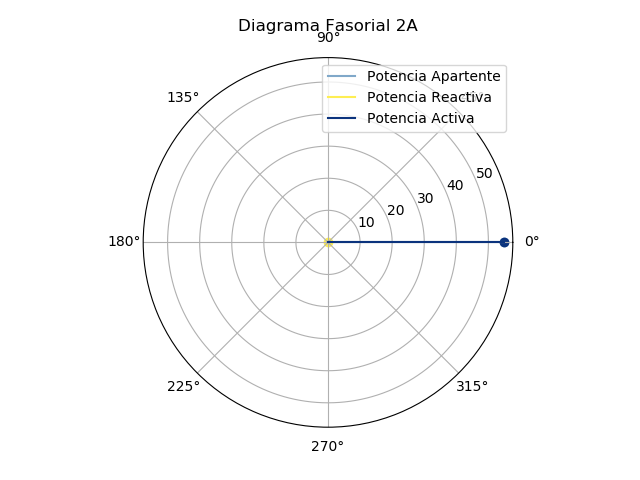
\includegraphics[width=1.2\linewidth]{Diag-Fas-2A}
  \caption{Circuito R.}
\end{minipage}%\\
\begin{minipage}{.5\textwidth}
  \centering
  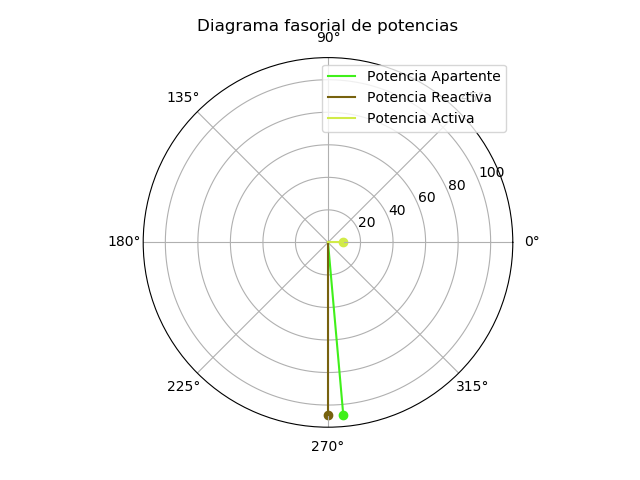
\includegraphics[width=1.2\linewidth]{Diag-Fas-2B}
  \caption{Circuito C.}

\end{minipage}\\
\begin{minipage}{.5\textwidth}
  \centering
  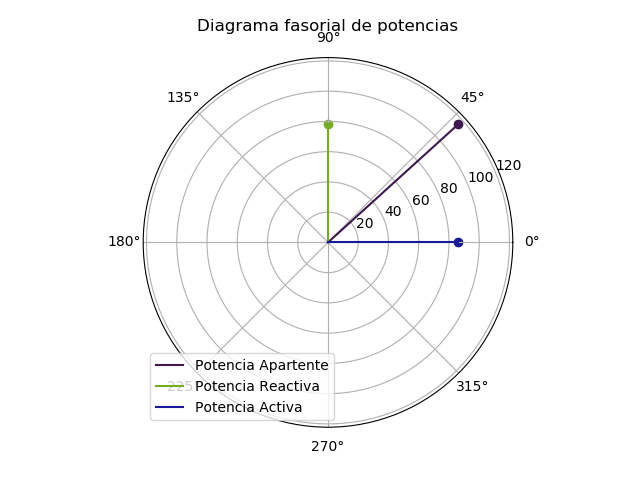
\includegraphics[width=1.2\linewidth]{Diag-Fas-2C}
  \caption{Circuito RLC.}
\end{minipage}
\end{figure}

\subsection*{\underline{Ejercicio 3}}
La finalidad de la tercer etapa del trabajo consistió en variar el factor de potencia del circuito de la figura (\ref{fig:2b}) a un valor de $ 0.9 $ mediante la adición de capacitores en paralelo. En un principio se agregó un total de $ 16 \ \mu F$, lo que implicó que $ cos \left(\varphi \right) = 0.74 $. Al subir la capacitancia en paralelo a $ 24 \ \mu F$, se observo que $ cos \left(\varphi \right) = 0.91 $.

\subsection*{\underline{Ejercicio 4}}
Por último, en la sección final de este trabajo, se buscó determinar analíticamente el valor capacitivo del banco de capacitores que se debería colocar en paralelo a los circuitos del ejercicio 2 para alcanzar un factor de potencia de $ 0,9 $. Realizando las cuentas adecuadas se obtiene
\begin{table}[H]
\centering
\begin{tabular}{|c|c|c|c|}
\hline
\textbf{Circuito} & \textbf{R} & \textbf{C} & \textbf{RLC} \\ \hline
\textbf{C [$ \mu F $]}        & 1,05      & 22,16       & 18,07         \\ \hline
\end{tabular}
\caption{Capacidad necesaria para alcanzar un fator de potencia de $ 0,9 $.}
\end{table} 

\end{document}
